\begin{figure}[H]
\centering
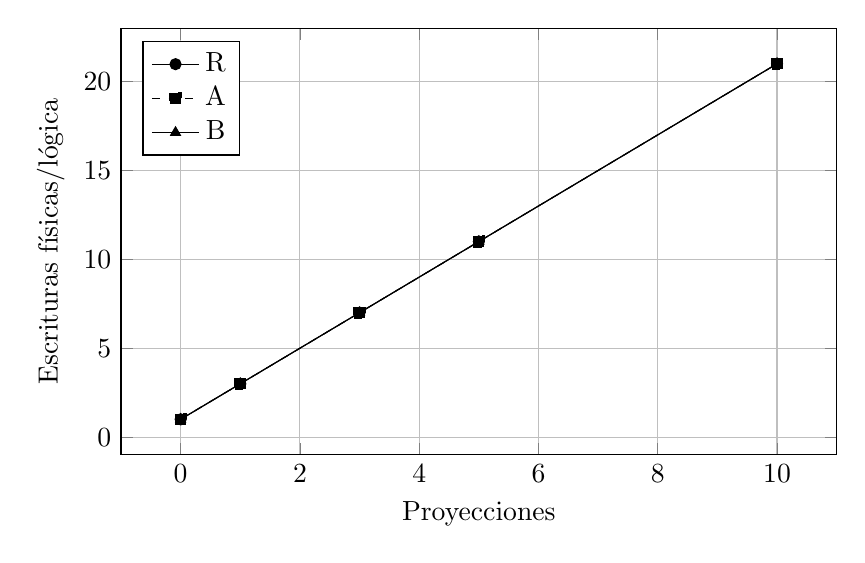
\begin{tikzpicture}
\begin{axis}[width=.88\textwidth,height=7cm,grid=major,legend pos=north west,
xlabel={Proyecciones},ylabel={Escrituras físicas/lógica},]
\addplot[black,mark=*,solid] coordinates {(0,1) (1,3) (3,7) (5,11) (10,21)};
\addlegendentry{R}
\addplot[black,mark=square*,dashed] coordinates {(0,1) (1,3) (3,7) (5,11) (10,21)};
\addlegendentry{A}
\addplot[black,mark=triangle*,solid] coordinates {(0,1) (1,3) (3,7) (5,11) (10,21)};
\addlegendentry{B}
\end{axis}
\end{tikzpicture}
\caption{Amplificación de escritura por número de proyecciones (N=10 000).}
\end{figure}